\chapter{Emscripten}
\label{cha:emscripten}

JavaScript is often called an assembly language of the Web.\footnote{http://www.hanselman.com/blog/JavaScriptIsWebAssemblyLanguageAndThatsOK.aspx} One could argue that since only one language is supported by browsers it could be made a compilation target similar to assembler for CPU. This statement is flawed since eventually JavaScript is translated to assembly making it only an intermediate step. Probably resemblance to ByteCode in JVM, which is compilation target of multiple languages like Java, Scala and Clojure is more in place.
Nevertheless, last years showed multiple projects aimed at converting code to JavaScript. Some introduce new syntax like CoffeeScript, Dart or TypeScript while still serving the same purpose - providing human readable code that is interpreted in browser on fly. Others, that are focus of this chapter, aim to convert existing projects to run in browser.

Several new projects are connected to make this happen. First steps in conversion between languages were made with LLVM project\footnote{http://llvm.org/} which currently is a collection of tools and compilers converting code to and from intermediate representation (LLVM IR). For C++ Clang\footnote{http://clang.llvm.org/} is a conversion tool.

\begin{figure}[h!]
  \caption{Pipeline of Emscripten conversion. Source: http://www.hanselman.com/blog/JavaScriptIsWebAssemblyLanguageAndThatsOK.aspx}
  \label{img:emscriptenpipeline}
  \centering
	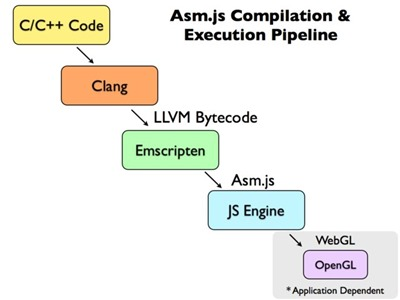
\includegraphics[width=8cm]{emscripten/pipeline.jpg}
\end{figure}

Code in LLVM is suitable for further conversion to language like JavaScript. This part is handled by Emscripten\footnote{https://github.com/kripken/emscripten/wiki} project. Initially compilation target for Emscripten was plain JavaScript. With recent developments asm.js\footnote{http://asmjs.org/spec/latest/} library was created. It provides syntax built on top of JavaScript, that is strongly typed and easily translatable to assembly language. All language specific annotations are added through bit NOP operations.

\lstinputlisting[caption=Example of code using asm.js,label=listing:asmjs]{emscripten/asm.js}

Project, built in cooperation with Mozilla Foundation, has its own engine for Firefox - OdinMonkey, designed to run faster for this limited and well-defined syntax.

Altogheter these projects resulted in multiple libraries and games converted from native version to JavaScript.

Proof-of-concept demo made in cooperation between Mozilla and Unreal is Epic Citadel HTML5 - Unreal Engine 3 technology demo\footnote{http://www.unrealengine.com/en/showcase/udk/epic\_citadel/}  instance running in browser.\footnote{http://www.unrealengine.com/html5/} Companies claim it took only four days to complete the conversion.

\begin{figure}[h!]
  \caption{Epic Citadel screenshot}
  \label{img:epicitadel}
  \centering
	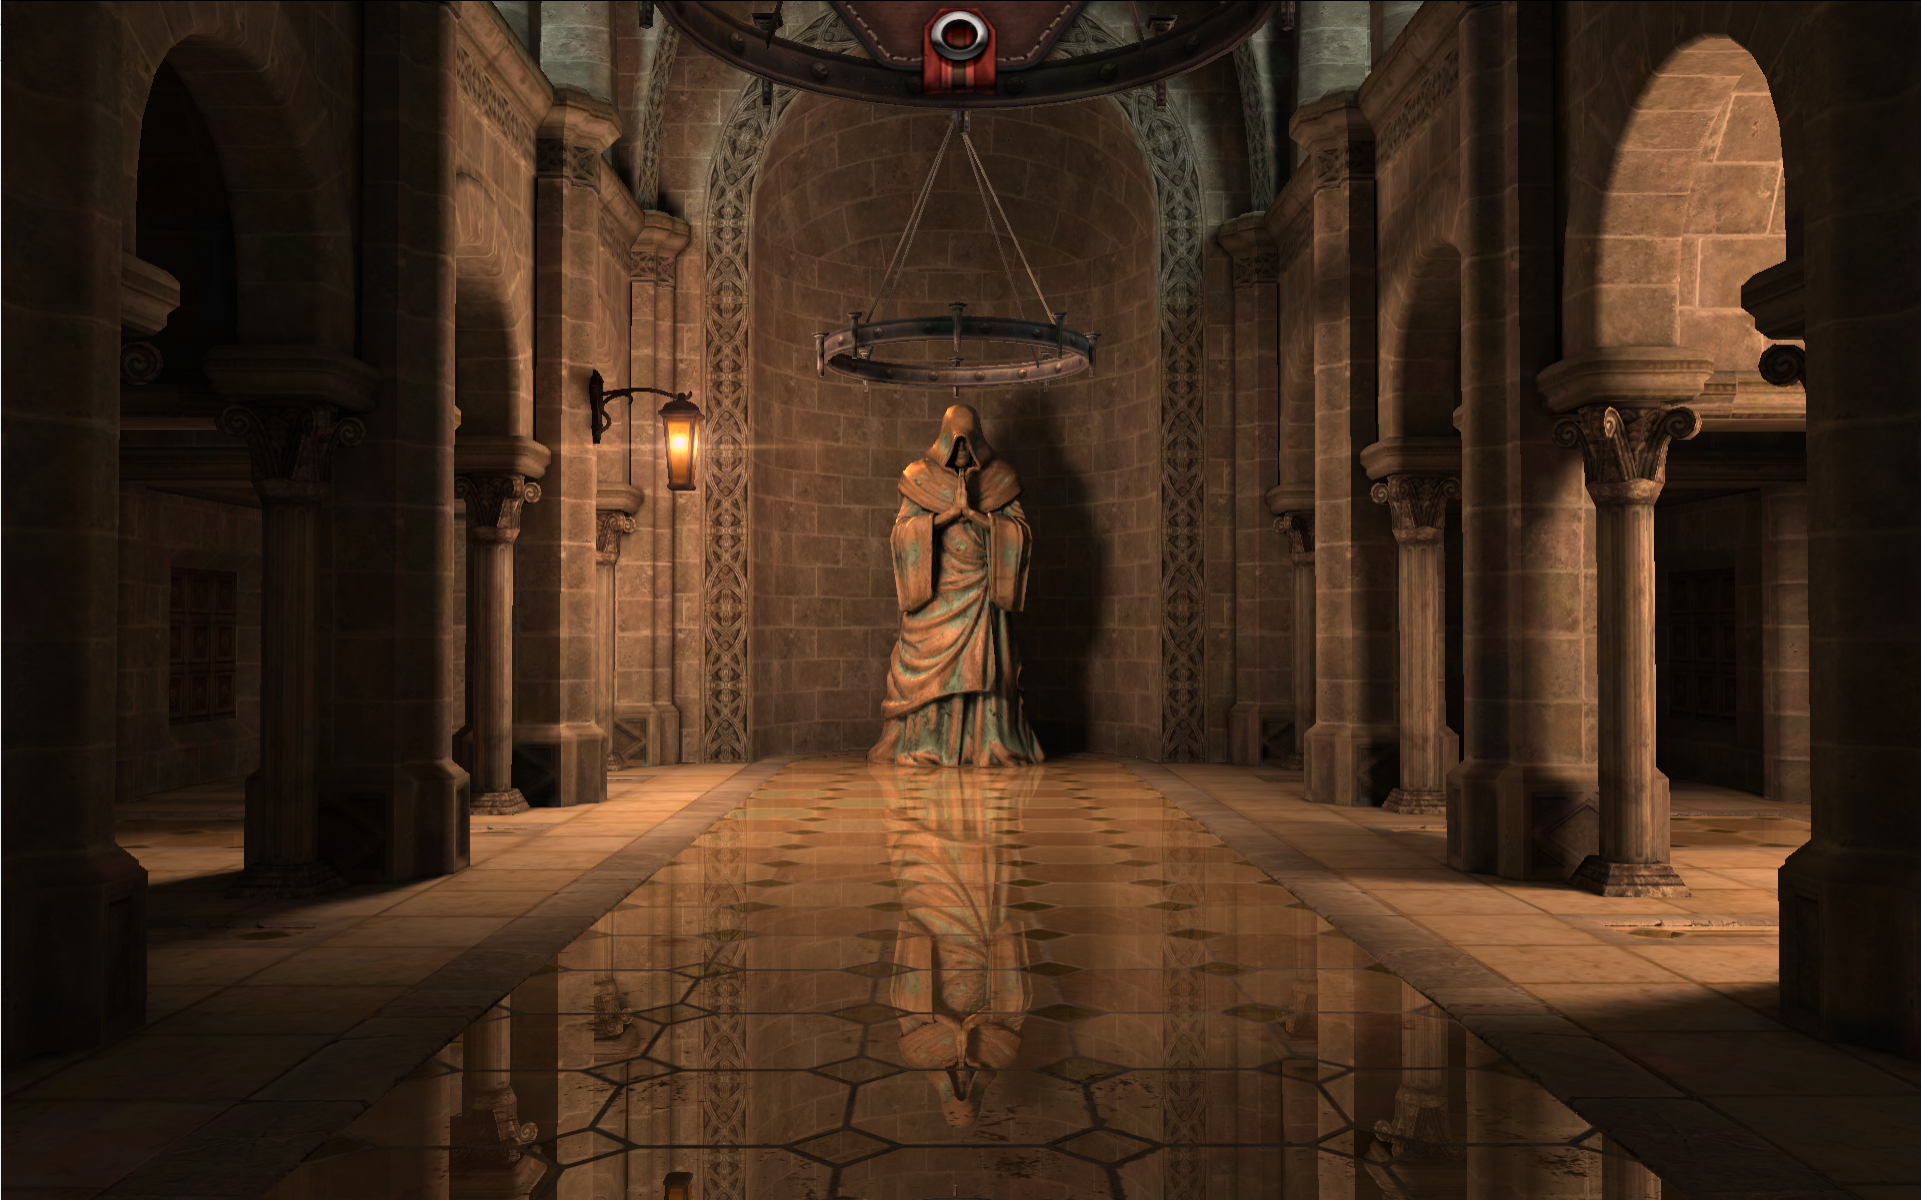
\includegraphics[width=16cm]{emscripten/epic-citadel.jpg}
\end{figure}

Another example of successful converted project is ammo.js\footnote{https://github.com/kripken/ammo.js/} - originating from Bullet physics engine.
TODO: Maybe extend this part a bit, cover more on how conversion was going and what were the issues.

\begin{figure}[h!]
  \caption{Ammo.js demo colliding 500 boxes at 30fps, available at http://kripken.github.io/ammo.js/examples/new/ammo.html}
  \label{img:epicitadel}
  \centering
	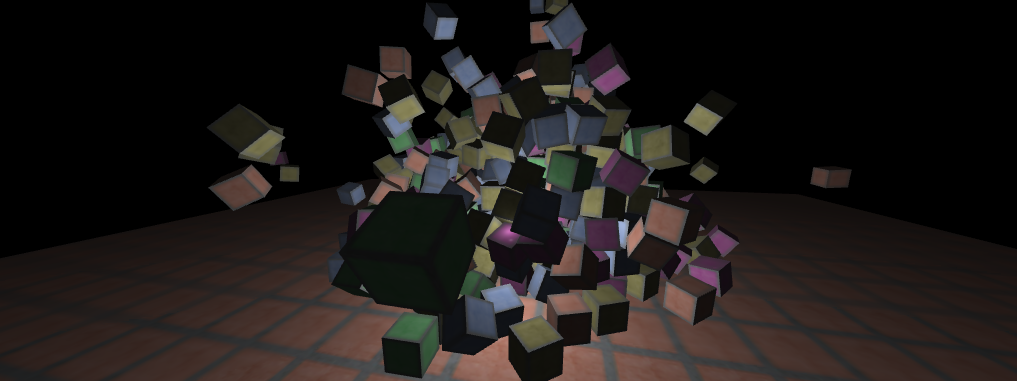
\includegraphics[width=16cm]{emscripten/ammojs.png}
\end{figure}

\section{Technology overview}
\label{sec:emscriptenoverview}

TODO: Explain static memory allocation in Float32Array and consequences for memory management.
TODO: Overview of asm.js modules, ahead of time compilation.


\section{Benchmarks}
\label{sec:embenchmarks}

TODO: Gather more benchmark results after codebase is frozen.
TODO: Summary of results - memory intensive demos work faster in Emscripten/asm.js, the ones with close to zero GC are faster in JS. Consider how usage of typed arrays would change results.

\begin{table}[h!]
\caption{Particle tests on different platforms}
\label{table:benchmarks}
\begin{tabular}{|p{4cm}||l|l|l||l|l|l|}
  	\hline
   Platform & \multicolumn{3}{c}{Unoptimised particles} & \multicolumn{3}{c}{Optimised particles}\\ \hline
   & C++ & JavaScript & Emscripten & C++ & JavaScript & Emscripten\\ \hline
   Fedora 19, Intel i7 2670QM, 4GB RAM, g++ 4.8.1 & 3.21s & 19.51s & 4.85s & 1.63s & 4.96s & 5.10s \\ \hline
   Windows 7, Intel i7 2670QM, 4GB RAM, g++ 4.7.3, Cygwin & 3.21s & 20.45s & 6.18s & 1.47s & 3.28s & 5.39s \\ \hline
\end{tabular}
\end{table}

\begin{table}[h!]
\caption{Spheres tests on different platforms}
\label{table:benchmarks}
\begin{tabular}{|p{4cm}||l|l|l||l|l|l|}
   \hline
   Platform & \multicolumn{3}{c}{$O(n^2)$ spheres} & \multicolumn{3}{c}{Octree spheres}\\ \hline
   & C++ & JavaScript & Emscripten & C++ & JavaScript & Emscripten\\ \hline
   Fedora 19, Intel i7 2670QM, 4GB RAM, g++ 4.8.1 & 4.96s & 9.02s & 12.35s & 
3.44s & 14.14s & 11.20s \\ \hline
   Windows 7, Intel i7 2670QM, 4GB RAM, g++ 4.7.3, Cygwin & 9.26s & 10.79s & 11.19s & 13.87s & 13.19s & 9.71s \\\hline
\end{tabular}
\end{table}
